\section{Introduction}

In the chapter \ref{ch:OverView}, we used the data-types i.e. `std\_logic' and `std\_logic\_vector' to define `1-bit' $\&$ `2-bit' input and output ports and signals. Also, some operators e.g. `and' and `or' etc. were discussed. In this chapter, some more information is provided on these topics.

\section{Lexical rules}
VHDL is case insensitive language i.e. upper and lower case letters have same meanings. Further, 1-bit numbers are written in single quotation mark and numbers with more than 1-bit are written in double quotation mark, e.g. $'0'$ and $''01''$ are the valid notations. Also, VHDL is free formatting language (i.e. spaces can be added freely), but we use the python like approach to write the codes, as it is clear and readable. Lastly in VHDL, `$--$' is used for comments. 

\section{Library and packages}
In the tutorials, we use only two packages i.e. `std\_logic\_1164' and `numeric\_std' packages, which are approved by IEEE. Further, There are various other non-IEEE-standard packages available e.g. std\_logic\_arith' etc., which allow quick and easy coding with VHDL. Since these are not standardized library therefore it may result in compatibility issues in future. 


\subsection{`numeric\_std' package}
The `std\_logic\_1164' package contains the various data types e.g. `std\_logic', `std\_logic\_vector' and `integer' etc. But we can not control the size of the integer (default 32 bit size) and format (i.e. sign and unsigned) using this package. Further,  `Natural' data type is available in this package, which allows only `0' and positive integer values. 

To gain more control over integer values, `numeric\_std' package can be used which allows `sign' and `unsigned' integer values along with the size control. For example, if integer has values from 0-7 only, then we can define `unsigned' data type of width 3 as shown in Listing \ref{vhdl:typeConvertEx}.

Although Entity and Architecture declarations are discussed in Chapter \ref{ch:OverView}; but following are the some additional information about these declarations, 

\subsection{Entity declaration}
Entity can have three types of ports i.e. `in', `out' and `inout' as shown in lines 3-6 in Listing \ref{vhdl:entityDeclaration}. Note that last declaration does not contain `;' at the end (see line 6). Also, types with different port names, can be defined in separate lines as shown in line 3-4. This is helpful for writing comments for different ports. 
\begin{lstlisting}[language=Vhdl, caption=Entity Declaration, label= {vhdl:entityDeclaration}]
entity entityEx is      -- entityEx is the name of entity
port(
	a, b : in std_logic;  -- inputs for encoder
	c : in std_logic;     -- input for decoder
	d : inout std_logic;  -- inout
	y, z : out std_logic  -- out (no ';' in the last declaration)
); 
end entityEx; 			    -- end entity declaration 
\end{lstlisting}

\subsection{Architecture body}
Architecture declaration consists of name of the architecture and name of the entity as shown in line 1 of Listing \ref{vhdl:architectureBody}. It contains two parts i.e. `declaration section' and `body'. Declaration section is optional which is defined between architecture name and `begin' statement as shown in line 2. In declaration section signals, variables and constants etc. can be defined (line 2), whereas design-logics are defined in body (line 4-7). We already see the use of signals and design-logics in Chapter \ref{ch:OverView}; variables, constants are other data types are discussed in next section.

\begin{lstlisting}[language=Vhdl, caption=Architecture body, label= {vhdl:architectureBody}]
architecture arch_Name of entityEx is 
	signal s0, s1: std_logic;  -- declaration section
begin  -- begin architecture
	s0 <= (not a) and (not b);
	s1 <= a and b;
	
	z <= s0 or s1;
end arch_Name;  -- end architecture
\end{lstlisting}

\section{Data objects}
In this section two types of data-objects are discussed. 
\begin{enumerate}
	\item \textbf{Signals}: Signals can be seen as the intermediate connections for different ports. We already saw various signals in Chapter \ref{ch:OverView}, which are used to design the 1-bit and 2-bit comparators e.g. in Listing \ref{vhdl:comparator1Bit}, the signal `s0' and `s1' are used for 1-bit comparator. 
	
	\item \textbf{Constants}: Constants are the name provided to a specific data-type as shown in Section \ref{sec:Constants}. 
\end{enumerate}

\section{Data types}
In this section, commonly used data-types are discussed. Data types can be categorized in four ways i.e. Scalar, Composite, Access and File types. We discuss only two types i.e. scalar data type and composited data type. We can design fairly large and complex designs with these two types, as shown in this tutorial. Further, file types are used to read and write contents to files; and access types are similar to pointers in C and can not be synthesized. 

\subsection{Scalar types}
In the tutorials, we will use following two scalar types, 
\begin{enumerate}
	\item \textbf{Integer Types}: Integers can be defined using `integer' keyword. Various operations can be performed on integer data types i.e. addition, subtraction, division and multiplication. Further, division will not include the decimal values e.g. $5/2$ will be solved as 2 instead of 2.5, as shown in listing \ref {vhdl:scalarTypeEx}.
	
%	\item \textbf{Real}: Real includes all the integer and decimal numbers. Various operations can be performed on integer data types i.e. addition, subtraction, division and multiplication. Unlike integer, here division $5/2$ will solved as 2.5. 

	\item \textbf{Enumerated Types}: Enumerated data types have a set of user defined values, as shown in listing \ref {vhdl:scalarTypeEx}. 
	
\end{enumerate} 

\begin{explanation}[Listing \ref{vhdl:scalarTypeEx}]
	This listing contains the example of `integer' and `enumerated' data types. Since `out' port is not readable, therefore in line 9, `x' is define as `inout' port (instead of out), because we are reading the `x' in line 30 i.e `if ($x>=0$)'.
	\\ \\
	In the current explanation `a=5' and `b=2' is assumed, as shown as comment in line 8. Lines 22-25 show the results for `integer' data type. The code is simulated using Modelsim and the results are shown in Fig. \ref{fig:scalarTypeEx}.  Note that division operation does not include the decimal value as shown in line 25 and in the figure.
	\\ \\
	Enumerated data type is defined in line 17 with name `stateTypes', which has two values i.e. `posState' and `negState'. Further, stateTypes, posState and negState are the user-defined name (not the keywords). Then in line 18, the signal `currentState' of type `stateTypes' is declared. Hence, `currentState' can have only two values i.e. posState and negState. 
	
	Process block at line 28 executes whenever there is any event on `x'. Line 30 checks whether x is greater than or equal to 0 and set the value to `posState, if condition is true; otherwise value is set to `negState'. Process block at line 37 executes whenever there is any event on `currentState' signal. If `currenState' is posState, then pA is set to 1; otherwise it is set to -1. In the current example, `x' is 3, therefore currentState and pA are set to posState and 1 respectively, as shown in Fig. \ref{fig:scalarTypeEx}.
	
	
\end{explanation}

\lstinputlisting[
language = Vhdl,
caption    = {Scalar data types},
label      = {vhdl:scalarTypeEx}
]{scalarTypeEx.vhd}

\begin{figure}[!h]
	\centering
	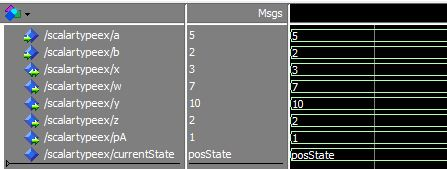
\includegraphics[scale=0.9]{scalarTypeEx}
	\caption{Scalar datatypes}
	\label{fig:scalarTypeEx}
\end{figure}

\subsection{Composite types}
The composite data types are the collection of values; which can be seen as `List' in python. In VHDL, list with same data types is defined using `\textbf{Array}' keyword; whereas list with different data types is defined using `\textbf{Record}'. VHDL examples of array and record are shown in Listing \ref{vhdl:compositeTypeEx}.

\begin{explanation}[Listing \ref{vhdl:compositeTypeEx}]
	In line 18, the array `newArray' is defined which can store 2 values (i.e. 0 to 1) of `std\_logic' type. Line 19 creates a signal `arrValue' of newArray type. Then in line 29 and 30, values are assigned to $0^{th}$ and $1^{st}$ position of `arrValue' signal. Finally at line 32, the value is assigned to z using $\&$ operator. $\&$ is known as Concatenation operator, which is discussed in section \ref{sec:opearators}.
	\\ \\
	Similarly, the record with name `newRecord' is defined in lines 21-25, with 4 items i.e. d1, d2, v1 and v2. In line 26, the signal `recordValue' of newRecord type is defined. Then in lines 35-39, values are assigned to recordValue signal. Finally, `and' operations are performed in lines 41 and 42, which are sent to output ports i.e. rY and rZ. 
	\\ \\
	Simulation results for the listing is shown in Fig. \ref{fig:compositeTypeEx}. 
\end{explanation}
\lstinputlisting[
language = Vhdl,
caption    = {Composite data types},
label      = {vhdl:compositeTypeEx}
]{compositeTypeEx.vhd}

\begin{figure}[!h]
	\centering
	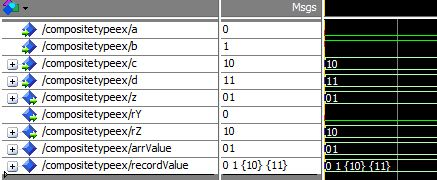
\includegraphics[scale=0.9]{compositeTypeEx}
	\caption{Composite datatypes}
	\label{fig:compositeTypeEx}
\end{figure}

\section{Operators}\label{sec:opearators}
In this section, various operators are discussed. 

\subsection*{Concatenation operators}
Concatenation operator is used to combine the two or more values e.g. [$'1'{ \ }\& { \ }'0' = { \ }''$$10''$] and [$''10''{ \ }\& { \ }'0' = { \ }''$$100''$]. Further, it is used at line 32 of Listing \ref{vhdl:compositeTypeEx}. 

\subsection*{Logical operators}
We already see some logical operators in previous examples e.g. `and' and `or' etc. VHDL provides 7 logical operators i.e. \textbf{and}, \textbf{or}, \textbf{not}, \textbf{nand}, \textbf{nor}, \textbf{xor} and \textbf{xnor}.

\subsection*{Relational operators}
In previous examples, we used various relational operators to check the conditions i.e. `=' and `$>=$'. VHDL provides 6 relational operations i.e. `=', `$>$', `$<$', `$>=$' (i.e. greater or equal), `$<=$' and `/=' (i.e. not equal to). 

\section{Type conversion}
VHDL is strongly typed language; in the other words, if we declare the two numbers e.g. `101' and `111' using two different data types e.g. `std\_logic\_vector' and `unsigned', then VHDL considers these numbers as different data types and we can not perform `or' and `xor' etc. operations directly on these two numbers. We need to convert the type of the number, to perform such operations as shown in line 18 of Listing \ref{vhdl:typeConvertEx}. Various conversion functions are shown in Table \ref{tbl:TableTypeConversion}, which is known as `Type Casting'.

\begin{table}
	\centering
	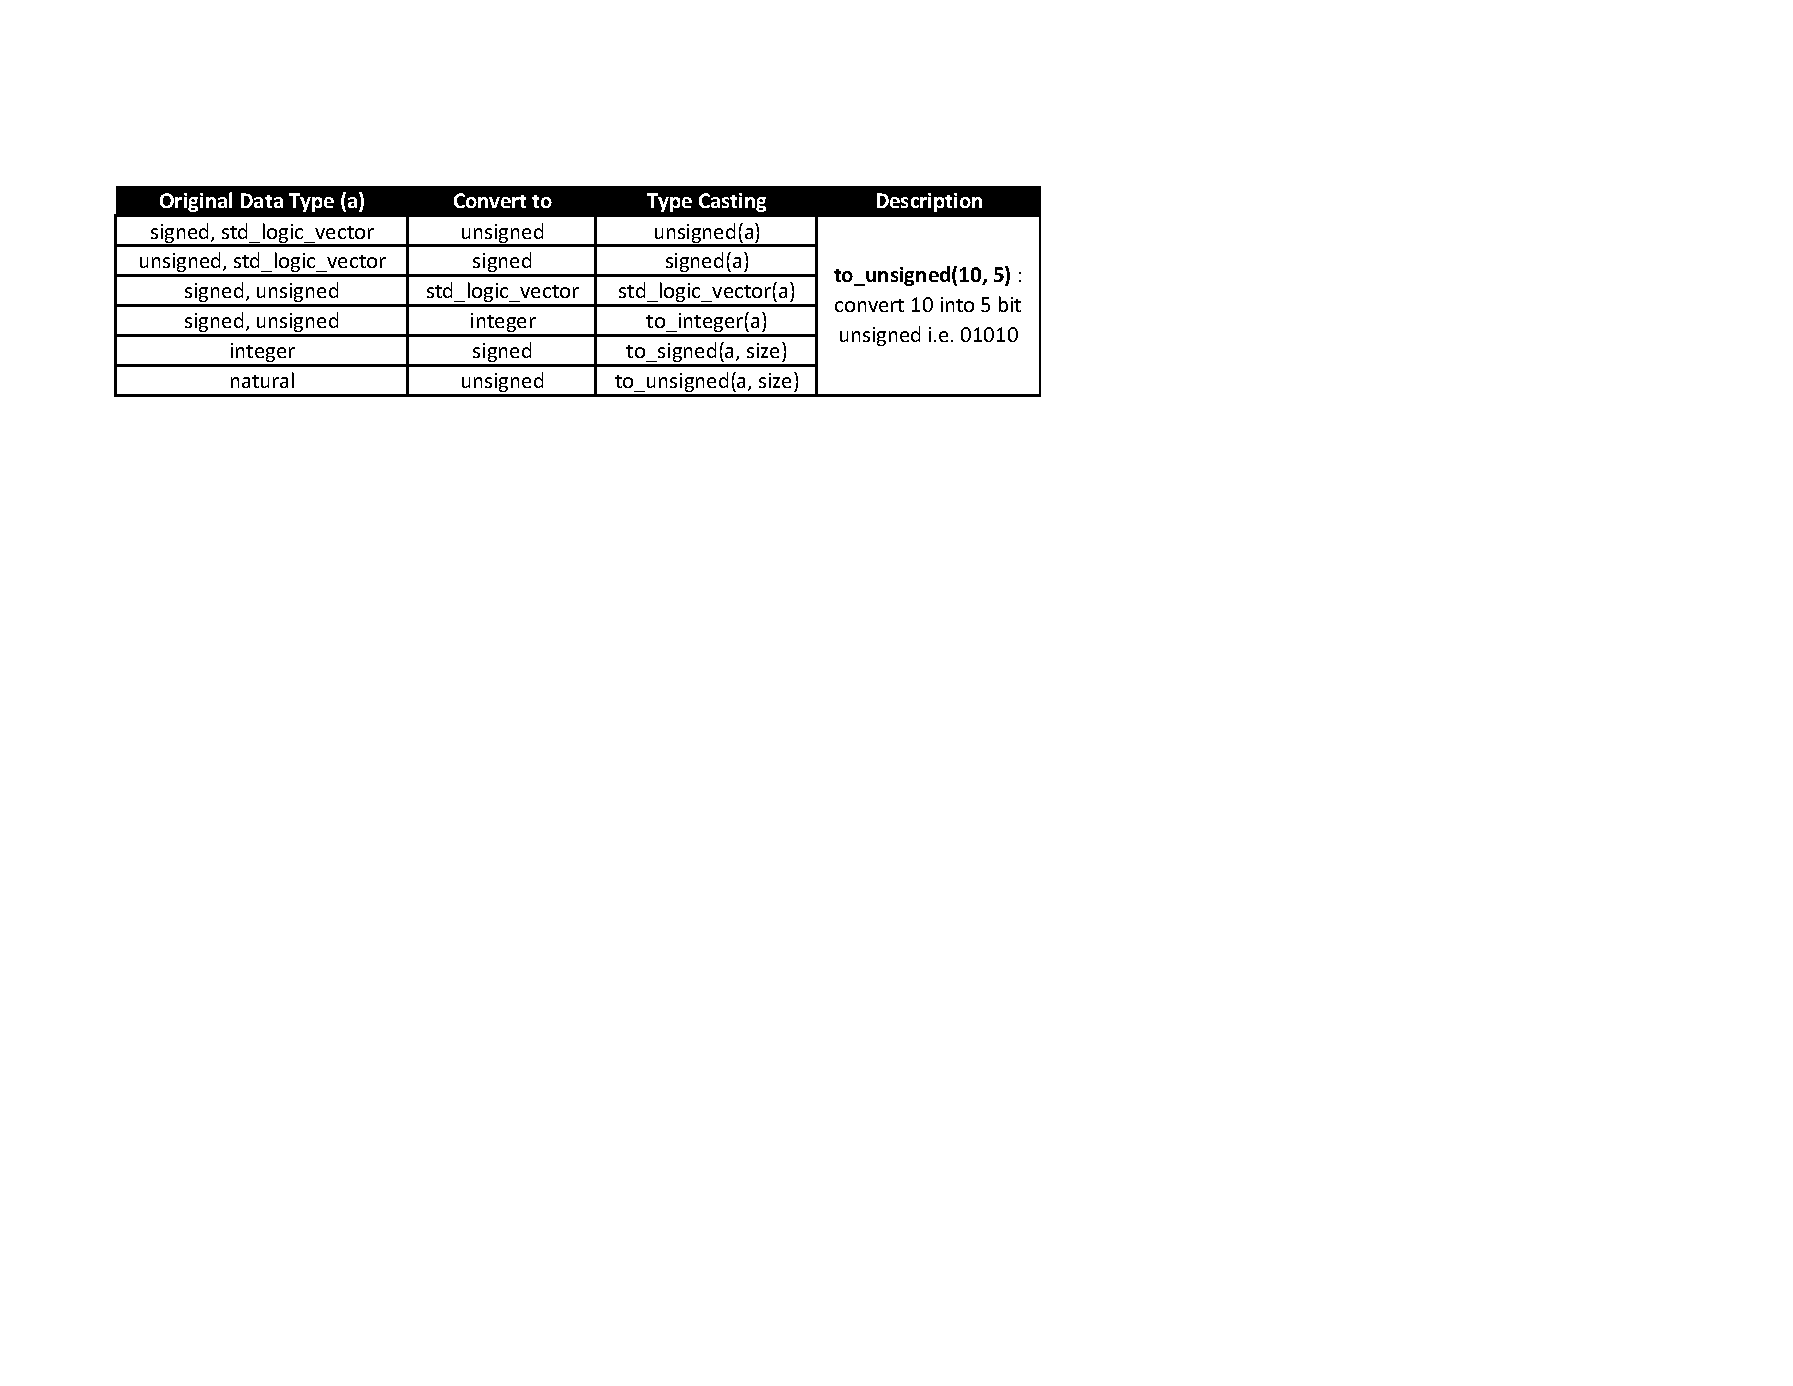
\includegraphics{TableTypeConversion}
	\caption{Type conversion}
	\label{tbl:TableTypeConversion}
\end{table}

\lstinputlisting[
language = Vhdl,
caption    = {Type conversion},
label      = {vhdl:typeConvertEx}
]{typeConvertEx.vhd}




\section{Constant and Generics}
Constant and Generics can be used to create reusable codes, along with avoiding the `hard literals' from the code as shown in following sections. 

\subsection{Constants}\label{sec:Constants}
Constants are defined in `architecture declaration' part and can not be modified in the architecture-body after declaration. In Listing \ref{vhdl:constantEx}, constant `N' is defined in line 14 with value 3. Then this value is used in line 15 and 16. Suppose we want to change the contant value to 4. Now we need to change the value from 3 to 4 in line 14 only (instead of changing everywhere in the code e.g. line 15 and 16 in this example). In this way, we can remove the `hard literal' from the codes.  

\lstinputlisting[
language = Vhdl,
caption    = {Constants},
label      = {vhdl:constantEx}
]{constantEx.vhd}

\subsection{Generics}
Generics are defined in `entity' and can not be modified in the architecture-body. VHDL code for generic is shown in Listing \ref{vhdl:genericEx}. Further, we can override the default value of generic during component instantiation in structural modeling style as shown in Listing \ref{vhdl:genericInstantEx}. 

\begin{explanation}[Listing \ref{vhdl:genericEx}]
	In Lines 7-10, two generics are defined i.e. `N' and `M'. Then ports `a' and `b' are defined using generic `N'. The process block (lines 20-27) compares `a' and `b' and set the value of `eq' to 1 if these inputs are equal, otherwise set `eq' to 0. 
\end{explanation}
\lstinputlisting[
language = Vhdl,
caption    = {Generics},
label      = {vhdl:genericEx}
]{genericEx.vhd}

\begin{explanation}[Listing \ref{vhdl:genericInstantEx}]
	In line 8, `x' and `y' are defined as 4-bit vector. Structural modeling is used in Line 15-17, where generic mapping and port mapping is done at line 16 and 17 respectively. 
	\\ \\
	Note that, in line 16 $N=>4$ will override the default value of N i.e. N=2 in Listing \ref{vhdl:genericEx}. Also, generic `M' is not mapped, therefore default value of M will be used, which is defined in Listing \ref{vhdl:genericEx}. In this way, we can remove `hard literals' from the codes, which enhances the reusability of the designs. 
\end{explanation}
\lstinputlisting[
language = Vhdl,
caption    = {Generic instantiation},
label      = {vhdl:genericInstantEx}
]{genericInstantEx.vhd}

\section{Conclusion}
In this chapter, we saw various data objects, data types and operators. Further, the two libraries i.e. `std\_logic\_1164' and `numeric\_std' are discussed. Generics and constants are shown which can be useful in creating the reusable designs. Lastly, since VHDL is strongly typed language therefore `type casting' is used for performing operations on two different data types. 